\documentclass[12pt]{standalone}
\usepackage{tikz}
\usetikzlibrary{automata,positioning}
\begin{document}
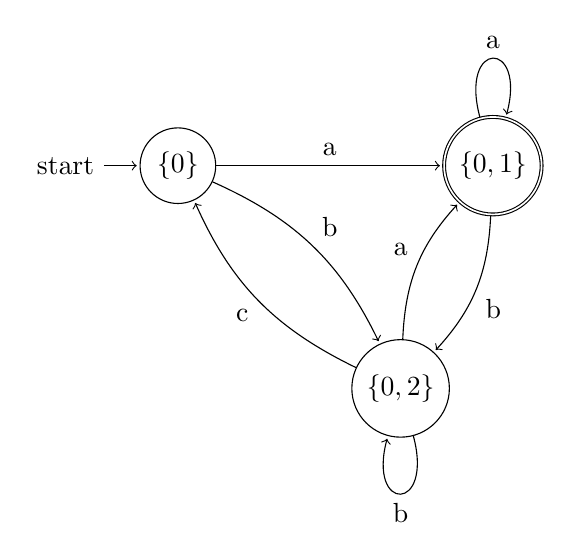
\begin{tikzpicture}[shorten >=1pt,node distance=4cm,on grid,auto] 
   \node[state,initial] (0)   {$\{0\}$}; 
   \node[state,accepting] (1) [right=of 0] {$\{0,1\}$}; 
   \node[state] (2) [below right=of 0] {$\{0,2\}$};

    \path[->] (0) edge  node {a} (1);
    \path[->] (0) edge [bend left = 20]  node {b} (2);
    \path[->] (1) edge [loop above] node  {a} (1);
    
    \path[->] (1) edge [bend left = 20] node {b} (2);

    \path[->] (2) edge [loop below] node  {b} (1);
    \path[->] (2) edge [bend left = 20] node {a} (1);
    \path[->] (2) edge [bend left = 20]  node {c} (0);
\end{tikzpicture}
\end{document}  

